%--------------------------------------||--------------------------------------%

\documentclass[11pt,letterpaper]{article} %  font size


%-----------------------------------PACKAGES-----------------------------------%

\usepackage[T1]{fontenc} % Choose an output font encoding (T1) that has support for the accented characters used by the most widespread European languages
\usepackage[utf8]{inputenc} % Allow input of accented characters (and more...)
\usepackage{graphicx} %  figures
\graphicspath{ {../../Figures/} {../Figures/} } % include images in the directory 'Figures' at the same level
\usepackage[round]{natbib} % names in citations
\usepackage{lineno} % line numbers
\usepackage{authblk} % allows more intuitive formatting for multiple authors/affiliations
\usepackage[margin=1in]{geometry} % make the margins 1 inch on all sides of the document
%\usepackage{amsmath} % useful for formatting math stuff, especially complex equations
%\usepackage{pdflscape} % rotate table into landscape mode
%\usepackage{subfigure} % side by side figures
%\usepackage{longtable} % for tables that span multiple pages.
\usepackage{setspace} % double spacing
\usepackage{float} % figure placement [H]


%----------------------------------FORMATTING-----------------------------------

%\topmargin -1cm %0.0cm
%\textwidth 16cm % what does this do?
%\textheight 21cm % what does this do?
%\footskip 1.0cm % what does this do?
%\oddsidemargin 0.0cm

\date{\today}
\doublespacing % initiate double spacing (package setspace)
%\linespread{2} % alternate method of double spacing


%------------------------------------TITLE--------------------------------------

\title{33 celebrity mansions you never even knew were haunted \\
(\textit{You won't believe number 17!})}

%-----------------------------------AUTHORS-------------------------------------

% using package 'authblk':
\author[1]{First Author\thanks{first.author@funstuff.com}}

\author[1,2]{Second Author}

\author[2]{Third Author}

% Make sure authors specify department, institution, and address.
\affil[1]{Department of Computer Science, \LaTeX\ University}
\affil[2]{Department of Mechanical Engineering, Superfabulous University}

% This is a janky way of doing authors, but avoids extra packages if you're into that.
%\author{
%	First Author\\
%		\small{\textit{First Author Affiliation}}\\
%		\small{\textit{firstauthor@affiliation.com}} \and
%	Second Author\\
%		\small{\textit{Second Author Affiliation}}\\
%		\small{\textit{secondauthor@affiliation.com}}
%	}

%---------------------------------REVIEWERS-------------------------------------
% Be sure to think of at least three reviewers to suggest to the journal
% Pro tip: look in the bibliography.
% 1. Reviewer1name ; reviewer1@email.com; title of relevant manuscript
% 2. Reviewer2name ; reviewer2@email.com; title of relevant manuscript
% 3. Reviewer3name ; reviewer3@email.com; title of relevant manuscript

%----------------------------------FORMATTING-----------------------------------
\begin{document}
\maketitle


%----------------------------------KEYWORDS-------------------------------------
\section*{Keywords}
Stuff, things, neat, cool, wow, instafun, tags4likes, etc

\linenumbers % start line numbers
\def\linenumberfont{\normalfont\small\rmfamily} % change line number font

% \pagebreak
%----------------------------------ABSTRACT-------------------------------------
\section*{Abstract}
This is the text of the abstract.
Abstracts should always be written after you've finished everything else.

%---------------------------------INTRODUCTION----------------------------------
\section*{Introduction}
For time immemorial, humankind has wondered: If I have two apples, and someone gives me another two apples, how many apples do I have? Some people did this \citep{Darwin1859}. Other people did that \citep{Wallace1869}.

The major problems with those approaches are that they forgot Poland.
We seek to remedy this by applying a Bayesian Approach.

%-----------------------------------METHODS-------------------------------------
\section*{Methods}
We constructed the following mathematical model (equation \ref{my_equation_label}) to better understand the concept:
% using '\ref{something}' in the text will refer to any object (e.g. figure, equation, table) which contains the corresponding '\label{something}'
% Note that you need to run latex a few times to get it to register numbers correctly

\begin{equation}\label{my_equation_label}
	Y = 2a + 2a
\end{equation}

Where $a$ represents an apple.

%-----------------------------------RESULTS-------------------------------------
\section*{Results}
We found that if you have two apples, and someone gives you another two apples, you have four apples.

%----------------------------------DISCUSSION-----------------------------------
\section*{Discussion}
Boy those results sure are neat. Now, the pressing question becomes: How do you like them apples? Further research is needed.

%-------------------------------ACKNOWLEDGEMENTS--------------------------------
\section*{Acknowledgements}
We wish to thank all of the little people.

%-----------------------------------FUNDING-------------------------------------
\section*{Funding}
% Specificy granting agency, grant number, and the recipient.
This study was funded by grant number 8-6753-09 from The Super-Rich Uncle Foundation to First Author.

%--------------------------------CONTRIBUTIONS----------------------------------
\section*{Author Contributions}
Conceived and designed the experiments:
Collected the data:
Conducted the analyses:
Wrote the first draft:
Edited the manuscript:

%-----------------------------------ETHICS--------------------------------------
\section*{Ethics Statement}
The authors declare big, honkin' conflicts of interest.

%----------------------------------REVIEWERS------------------------------------
% A list of recommended reviewers.

%-------------------------------------DATA-------------------------------------%
\section*{Data Availablity}
% Are the data and code available in a permanent, publicly accessible data archive or repository?
The data and code used to generate our results can be found at the following url:


%----------------------------------REFERENCES-----------------------------------
%\section*{References} % commented out because the section title is automatically inserted if using an automatically-generated bibliography

\bibliographystyle{apalike} % or: plain,unsrt,alpha,abbrv,acm,apalike,ieeetr
\bibliography{my_cool_refs} % path to your .bib file excluding .bib extension (e.g. /Users/threeprime/Documents/Publications/bibtex/library)


%-----------------------------------FIGURES-------------------------------------
\pagebreak
\section*{Figures}

\begin{figure}[h!] % [h!] forces the figure to be placed roughly here
  \centering
    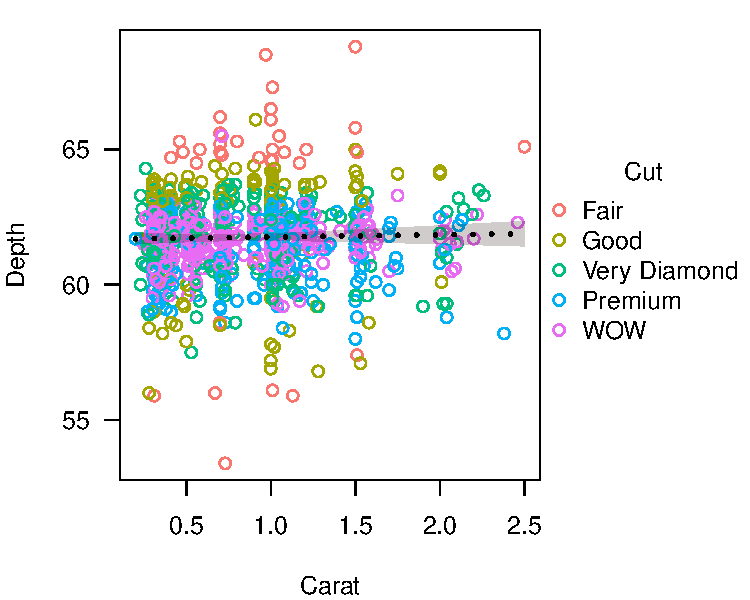
\includegraphics[width=1\textwidth]{depth_by_carat.pdf}
    \caption{\protect\input{../../Figures/depth_by_carat_legend.txt}}
%    \begingroup
%    \obeylines
%    \endgroup
  \label{depth_by_carat} % use this to refer to your figure in the text, so that numbering updates automatically
\end{figure}


%----------------------------------SUPPLEMENT-----------------------------------
\pagebreak
\section*{Supplemental Material}

Here is some other junk we tried.





\end{document}
